\label{chap_structure}

In Sec.~\ref{sec_conduction} and~\ref{sec_source_term} {\psiboil} programs
were used to solve transport equations for steady heat conduction. 
%
Although these problems are simple, the programs which were
developed ({\tt 07-01-main.cpp} and {\tt 07-03-main.cpp}) featured
a general structure {\psiboil} programs assumes, if used for
simulating general transport phenomena. 

Since this structure is typical also for simulating much more complex 
phenomena, it is outlined here as a reference point for programs
developed in later chapters. 
%
Figure~\ref{fig_structure} shows the typical structure of a {\psiboil}
program. The program flows from top to bottom and is divided into six
logical units (numbers 1-6 on the left of Fig.~\ref{fig_structure}) in
addition to header (H) and footer (F). The structures on the left
side of~Fig.~\ref{fig_structure} illustrates the actions performed, and
most of them are connected by a straight line with {\psiboil}'s classes 
(or global objects) which perform or define them. There are 
{\em dependencies} between the classes. For example, {\tt Domain}
created from three {\tt Grid1D}'s (Sec.~\ref{sec_domains}), meaning
that {\tt Domain} depends on {\tt Grid1D}. These dependencies govern
the order in which {\psiboil}'s objects are created. There is some
flexibility in the order objects are used in the general structure.
But, thick dashed lines should not be crossed, except for objects
with dashed frame. For example, simulation time ({\tt Times}) is now
in unit~3, but since it does not depend on any other object, it could
have been defined right after the header. That is illustrated with the
small dashed arrow on the left, and with the small letter H next to it.
In the same way, variable initialization, now performed in unit~5, 
could have been done right after the variable definition, as denoted
by the small arrow and number~2. On the other hand, multigrid solver~{\tt AC}
from unit~5, can {\em not} be defined before the governing equations
in unit~4 and therefore can {\em not} cross the dashed line. 

%-------------%
%             %
%  Structure  %
%             %
%-------------%
\begin{figure}[ht]
  \centering
  \setlength{\unitlength}{1mm}
  \begin{picture}(130,195)(0,0)
    \thickbox{130}{195}
    \put(0,0){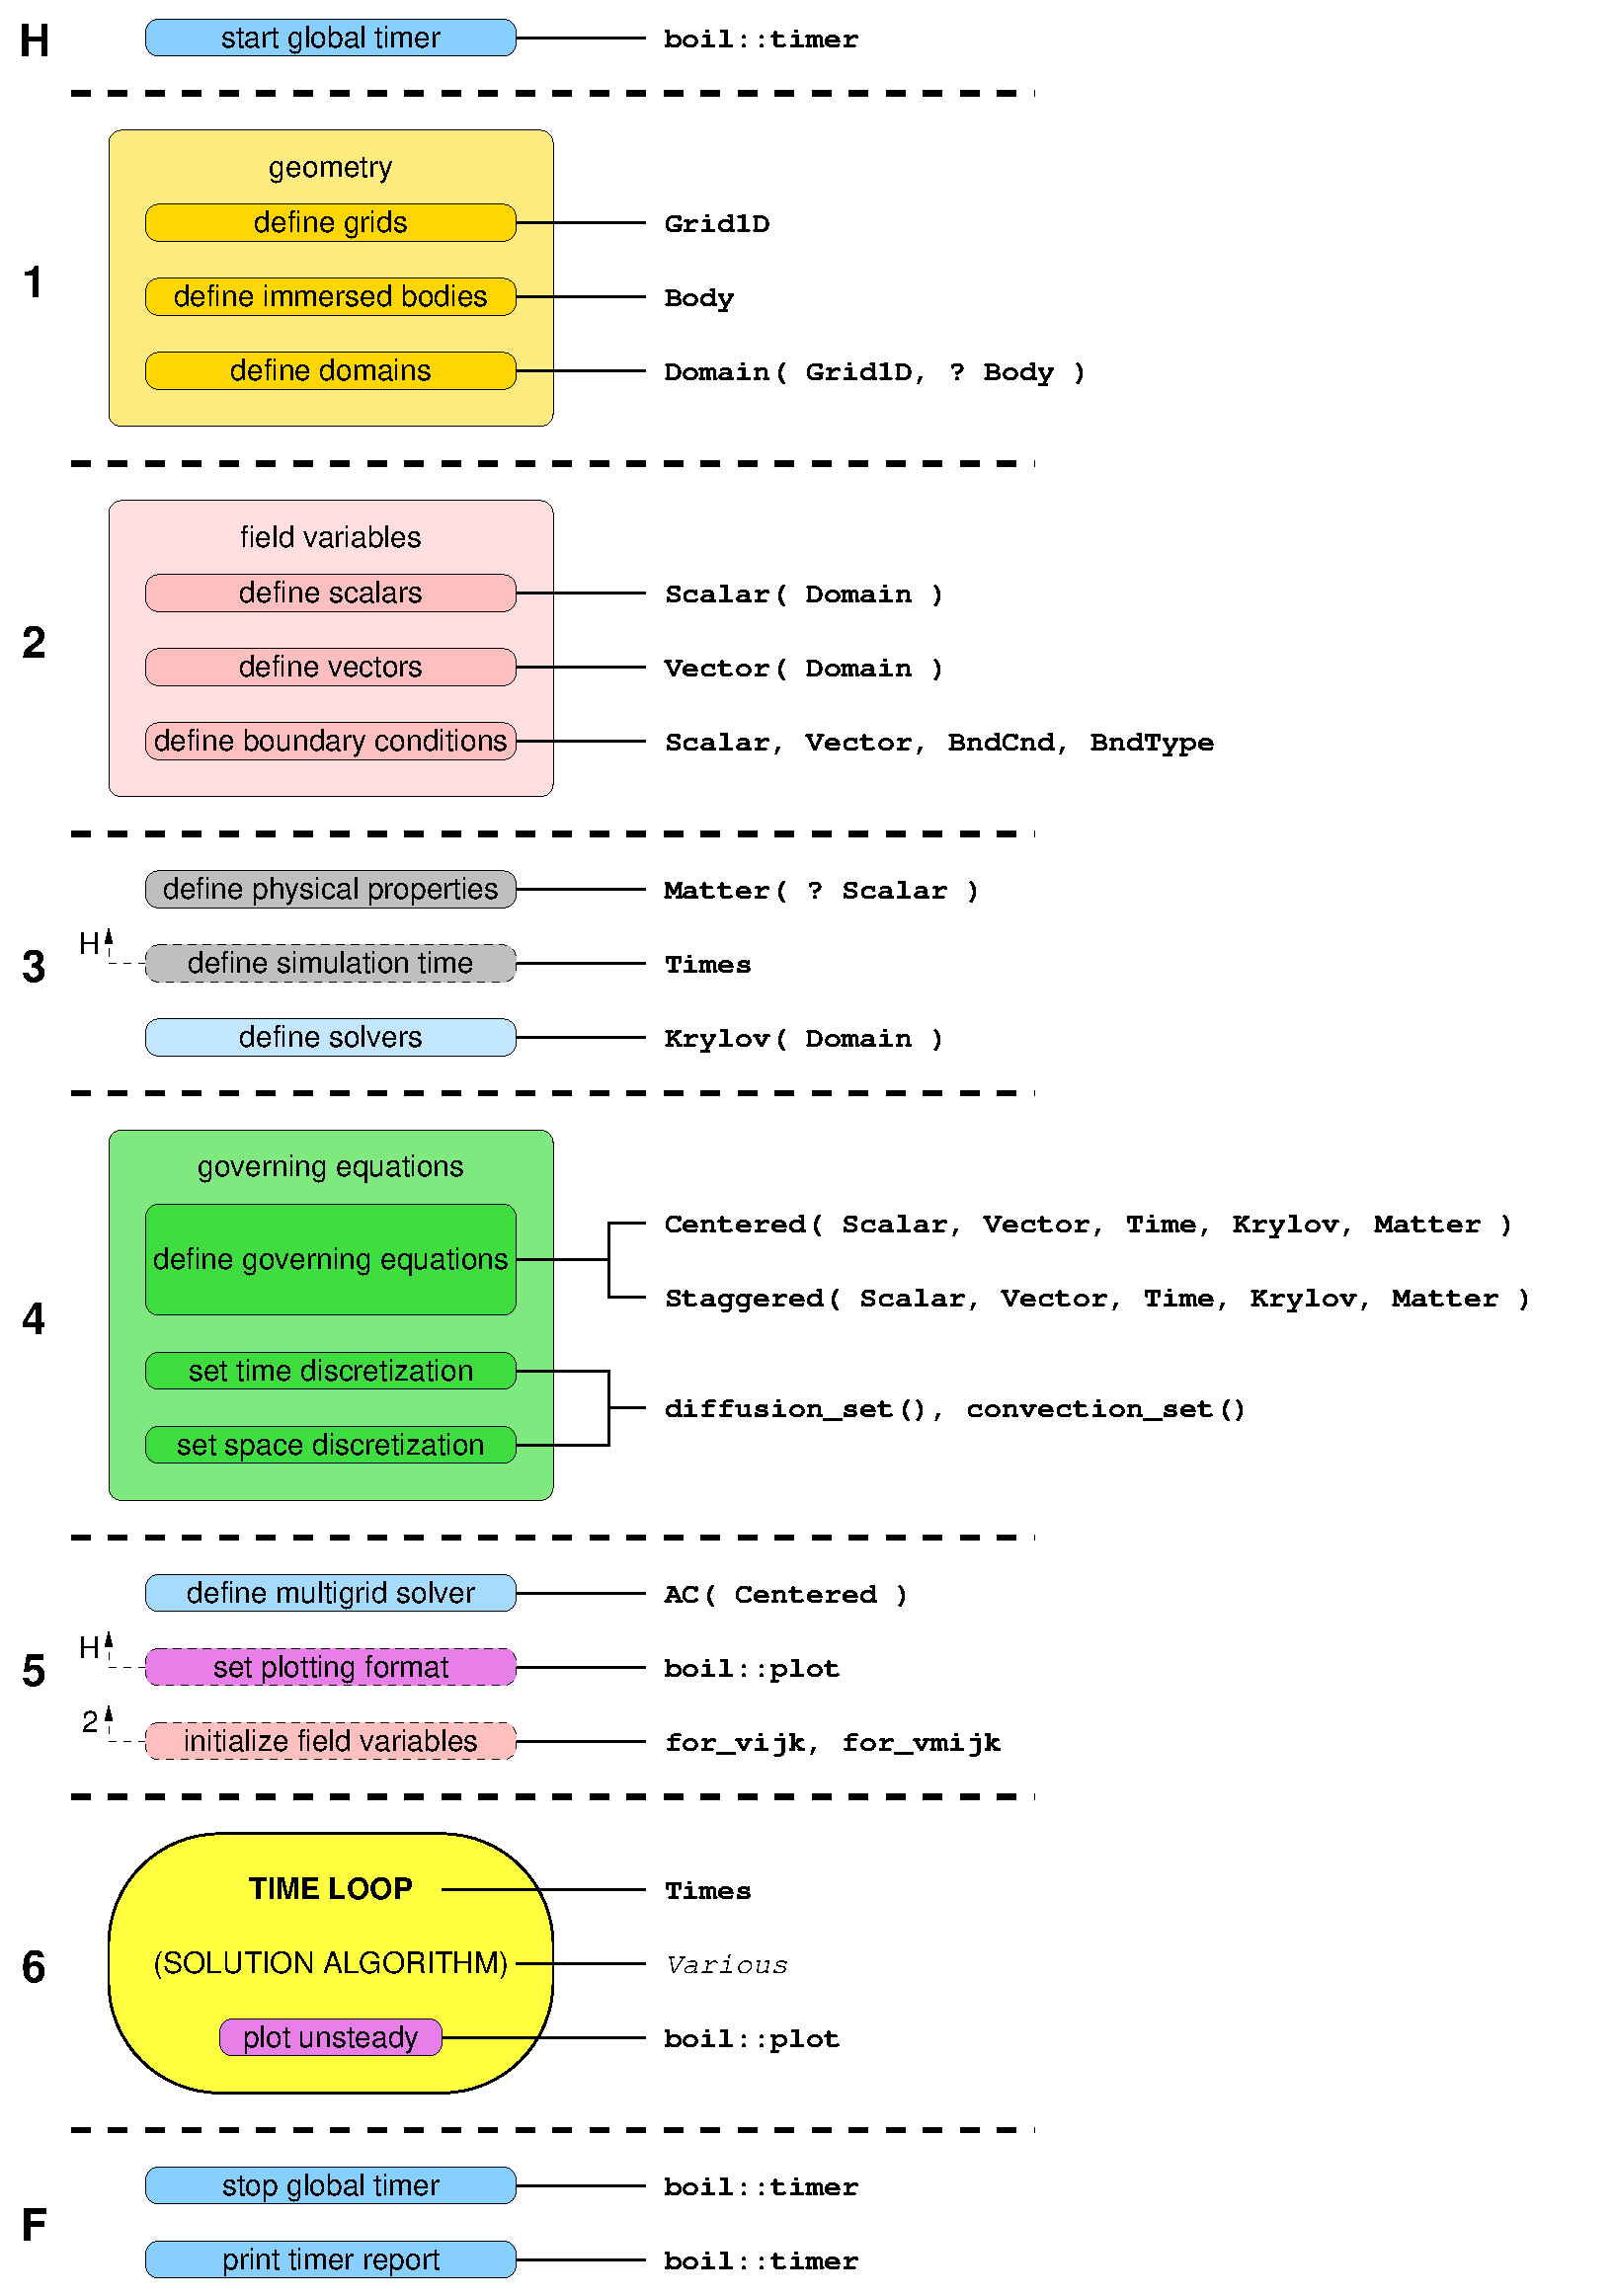
\includegraphics[scale=0.5]{Figures/08-01-structure.eps}}
  \end{picture}
  \caption{General structure of a {\psiboil} program.}
  \label{fig_structure}
\end{figure}

Header~(H) starts global object {\tt boil::timer}, while footer~(F)
stops it and prints the information on the CPU time on the terminal.
Header and footer must be present in every {\psiboil} program, because
many object use local timers to measure the performance of their
member functions. 

Quite naturally, right after the header, first unit starts which defines 
geometry (enclosed in an orange frame on~Fig.\ref{fig_structure}). 
Definition of geometry means defining grids ({\tt Grid1D}), IB's 
({\tt Body}) and domains ({\tt Domain}). 

Once the computational domain is defined, we can proceed with definition
of scalar and vector fields ({\tt Scalar} and {\tt Vector}) featured
in transport equations being solved. As soon as their are defined,
boundary conditions should be imposed on them as well. 

Third unit is a bit heterogeneous. It defines physical properties ({\tt Matter})
which depends on {\tt Scalar} in case of multiphase flows\footnote{That will
be covered in later chapters.}. Simulation time is also placed in this unit,
although it could have been defined right after the header. We prefer to put
it here for convenience, just to be closer to governing equations unit which
uses it as a parameter. Finally, solvers {\tt Krylov} are quite rigidly in
this unit. They must be defined after field variables and before governing
equations. 

Unit number four is dedicated to definition of governing equations. All the
equations are defined here (usually, that means: {\tt Momentum}, {\tt Pressure},
{\tt Enthalpy} \dots) as well as particular details about spatial and
temporal discretization. As far as spatial discretization is concerned,
various convection schemes can be defined (see the global class {\tt Limiter}
and associated ravioli class {\tt ConvScheme} in the directory: {\tt Src/Global}).
This feature is yet to be explored in the chapters below. Temporal discretization
schemes have been briefly touched upon in~Sec.~\ref{sub_sec_time_stepping}.

The following unit, number five, is actually a preparation for the time-loop.
As first, a multigrid solver ({\tt AC}) has to defined and it depends on the governing
equations. {\tt AC} is almost invariantly defined for pressure, while the other
variables, particularly when discretized for unsteady simulation, have 
well-conditioned linear systems and {\tt Krylov} solvers are usually efficient 
enough. Variables and source terms should be initialized before the time loop,
as well as plotting format. Both of these last two object could have been
defined much sooner. Variables could have been initialized right after their
definition, while the plotting format could have been chosen right after the
header (indicated with small arrows). 

Undoubtedly, the most important unit of the {\psiboil} is unit six,
the {\em Time loop}. It can be as simple as a single call to linear
solver\footnote{For example, line~38 in {\tt 07-01-main.cpp} is a complete
{\em Time loop}.} or as complex as time loop embedding another 
iterative procedure to couple various equations. This unit will vary
the most between different programs and different classes of problems
in particular. Therefore, it is beyond the scope of this chapter to
explain it any further. 

General structure of a {\psiboil} program, resembles two things: an
{\em input file} for a CFD package defining the problem to be solved 
(defining geometry, boundary conditions, material properties, choosing
plotting format, \dots), but also a flow diagram of a CFD program. 
In essence, it serves as both. As stated in Sec.~\ref{sec_about},
each problem solved with {\psiboil} requires a separate main program
(stored in {\tt main.cpp}), which used {\psiboil}'s objects to solve
a particular program. Each program defines geometry, boundary condition,
physical properties (units 1-4 in Fig.~\ref{fig_structure}), typical for 
an input file, but also defines the algorithm (units 5 and 6 
in Fig.~\ref{fig_structure}), as the flow diagram does. 
%
% really? When explaining the programs in the following chapters, we will try to
% really? explain them in parts corresponding to units introduced in this chapter. 

%---------------------------------------------------------------------nutshell-%
\vspace*{5mm} \fbox{ \begin{minipage}[c] {0.97\textwidth} %-----------nutshell-%
    {\sf Chapter \ref{chap_structure} in a nutshell} \\  %------------nutshell-%
   
      - Although {\psiboil} should be regarded as a collection of objects which
      facilitates the building of programs for numerical analysis of transport
      phenomena, each such program has a typical structure, represented
      in this chapter in form of a diagram. \\

      - The typical structure has six distinct units, in addition to header
      and footer. \\

      - This structure is flexible to some extent, but dependencies between
      the units introduce a certain order in which {\psiboil} objects are 
      laid out. \\

      - {\psiboil}'s main program (the one which is different for each problem
      solved) can be regarded as an input file for simulation and a flow
      diagram of the applied algorithm.

  \end{minipage} } %--------------------------------------------------nutshell-%
%---------------------------------------------------------------------nutshell-%
